\documentclass[12pt,a4paper]{article}

\usepackage{polski} % Kodowanie znaków zostało wykonane w UTF-8 
\usepackage{indentfirst}
\usepackage{graphicx}
\usepackage{fancyhdr}
\usepackage{lastpage}
\usepackage{hyperref}
\usepackage{biblatex}

\title{Specyfikacja funkcjonalna projektu grupowego z przedmiotu \textit{Algorytmy~i~struktury~danych}}
\author{Krzysztof Kowalski, Szymon Motłoch, Aleksander Wodnicki}
\date{17 grudnia 2020}

\begin{document}
\maketitle
\thispagestyle{empty}
\newpage
\pagestyle{fancy}
\fancyhf{}
\rhead{Specyfikacja funkcjonalna projektu grupowego z przedmiotu \textit{AiSD}}
\rfoot{Strona \thepage \hspace{1pt} z \pageref{LastPage}}
\tableofcontents
\newpage

\section{Wstęp}
\subsection{Cel dokumentu}
Niniejszy dokument zawiera informacje na temat tworzonej aplikacji w~ramach projektu grupowego z przedmiotu \textit{Algorytmy i struktury danych}. Opisuje on zasady działania programu, tj. sposób uruchomienia, przyjmowane dane, sposób działania, a także dane wyjściowe otrzymywane po jego zakończeniu. Co więcej, opisuje on sposób testowania programu oraz interpretację komunikatów o błędach. W skrócie – użytkownik, po zapoznaniu się z tym dokumentem, będzie w stanie bez problemu uruchomić omawiany program i~posługiwać się nim.

\subsection{Cel projektu}
Celem projektu jest utworzenie aplikacji z interfejsem graficznym, która będzie przeprowadzała symulacje działania pracy pogotowia ratunkowego w czasach pandemii. Na bazie informacji znajdujących się w dostarczonych przez użytkownika plikach, zostanie utworzona mapa, a na niej umiejscowione osoby oczekujące na pomoc ze strony pogotowia. Na bazie informacji o tym, gdzie znajdują się szpitale oraz jakie istnieją drogi, pogotowie będzie przemierzać kraj w poszukiwaniu najbliższego szpitala, który nie został jeszcze odwiedzony przez karetkę. Celem tych podroży będzie znalezienie wolnego miejsca w szpitalu dla pacjenta.

\subsection{Opis symulacji}
W tej sekcji znajduje się szczegółowy opis teoretycznych założeń projektu, które definiują jak symulacja będzie przebiegać.

Naszą mapą jest najmniejszy zbiór wypukły zawierający w sobie wszystkie obiekty z pierwszego pliku. Po wygenerowaniu takiej mapy, umieszczamy na niej pacjentów według współrzędnych z drugiego pliku. Pacjenci będą rozwożeni w takiej kolejności, w jakiej znajdowali się w pliku. Jeśli pacjent został dodany pojedynczo poprzez podanie współrzędnych w oddzielnym formularzu, to będzie obsłużony jako ostatni.
    
W symulacji nie występuje ograniczenie ilości karetek. Dla każdego pacjenta, który pojawi się na terenie kraju, zostanie od razu rozdysponowana do niego karetka. W żaden  sposób nie zajmujemy się pacjentami poza granicami naszego kraju. Ponieważ pacjent może mieć współrzędne nieznajdujące się na zdefiniowanych drogach, karetka, która po niego przybędzie pokona drogę jadąc po linii prostej do najbliższego szpitala. Jeśli w szpitalu będzie znajdować się miejsce dla pacjenta, zostanie on do niego przyjęty i liczba wolnych łóżek znajdujących się w szpitalu zostanie pomniejszona. W przeciwnym razie, jeśli nie będzie miejsc w szpitalu, karetka będzie jeździć po kolejnych szpitalach i szukać wolnego miejsca dla pacjenta. Karetka nie będzie brała pod uwagę ilości wolnych miejsc w szpitalach, tylko odległość między nimi i to, czy zostały już wcześniej odwiedzone. Jeśli karetka odwiedzi wszystkie szpitale i nie znajdzie wolnego miejsca dla pacjenta, będzie stała pod ostatnim z odwiedzonych szpitali czekając aż zwolni się miejsce w tym szpitalu.

\section{Opis działania programu}
W tej sekcji zostaną opisane zagadnienia związane z działaniem programu, tj. sposoby i scenariusze uruchomienia, dane wejściowe, graficzny interfejs symulacji, jak również komunikaty błędów. 

\subsection{Opis graficznego interfejsu}
Tak wygląda poglądowy projekt graficznego interfejsu aplikacji. Poniżej opisane zostały wszystkie jego istotne elementy.

\begin{figure}[h!]
\centering
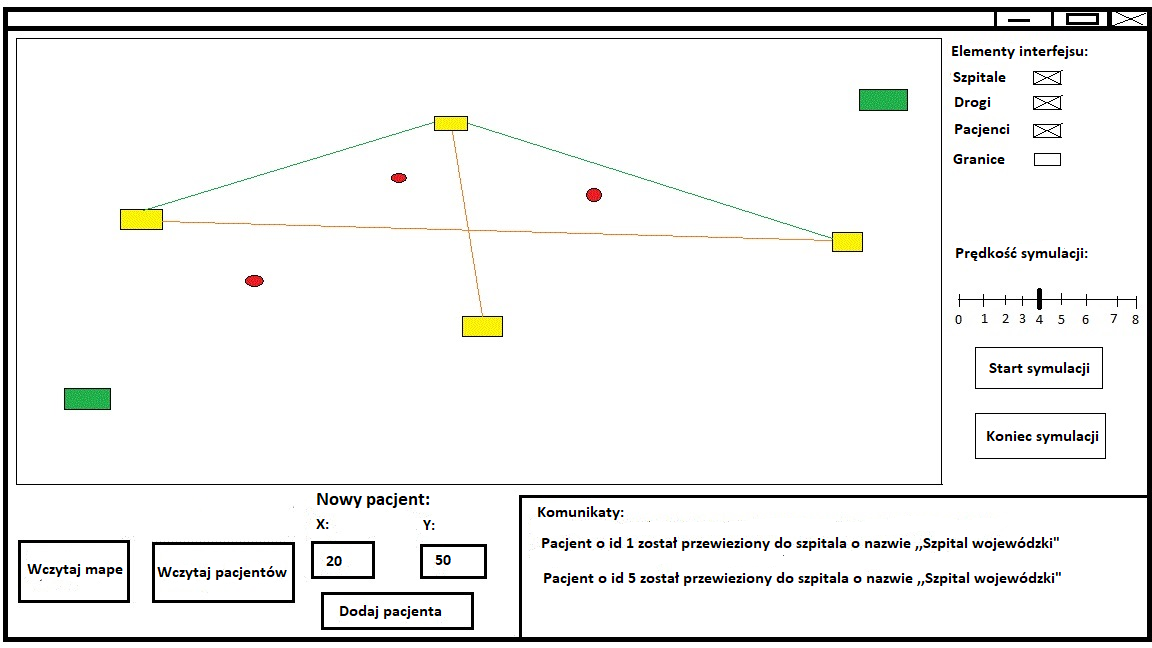
\includegraphics[width=1.0\textwidth]{GUI}
\caption{Projekt graficznego interfejsu gry} 
\label{fig:GUI}
\end{figure}

\begin{itemize}
\item \textbf{Wczytaj mapę} – przycisk służący do wczytania pliku z danymi o~szpitalach, obiektach i drogach;
\item \textbf{Wczytaj pacjentów} – przycisk służący do wczytania pliku ze współrzędnymi pacjentów;
\item \textbf{Nowy pacjent} – pole, w którym możemy dodać współrzędne nowego pacjenta bez konieczności wczytywania pliku;
\item \textbf{Dodaj pacjenta} – przycisk służący do dodania powyższego pacjenta, którego współrzędne wprowadziliśmy w odpowiednich komórkach do tego przeznaczonych;
\item \textbf{Komunikaty} – miejsce, w którym użytkownik będzie otrzymywał informacje o kolejnych etapach symulacji;
\item \textbf{Prędkość symulacji} – suwak służący do określenia prędkości, z jaką symulacja będzie przebiegać;
\item \textbf{Start symulacji} – przycisk służący do rozpoczęcia symulacji;
\item \textbf{Koniec symulacji} – przycisk służący do zatrzymania symulacji przed jej zakończeniem;
\item \textbf{Elementy interfejsu} – miejsce, w którym użytkownik może odznaczyć obiekty według swoich preferencji. Skutkuje to ich zniknięciem z mapy i może poprawić czytelności symulacji.
\end{itemize}

\subsection{Dane wejściowe}
Danymi wejściowymi, które powinien zapewnić użytkownik, aby możliwe było rozpoczęcie symulacji, są dwa pliki w formacie \texttt{.txt}. W obu plikach poszczególne sekcje powinny zostać rozdzielone odpowiednimi nagłówkami. Linia pliku, w której znajduje się nagłówek rozpoczyna się znakiem \texttt{\#}. Nagłówki powinny wyglądać identycznie jak nagłówki, które będą przedstawione w przykładach w dalszej części dokumentu. Ponadto, wartości w liniach powinny być podzielone na części separatorami \texttt{|}.

\newpage
\subsubsection{Plik z informacjami o mapie}
W pierwszym pliku wejściowym użytkownik będzie mógł zdefiniować elementy takie jak szpitale, obiekty oraz drogi. Na podstawie tego pliku będzie wygenerowana mapa, na terenie której przeprowadzona zostanie symulacja.
 
\begin{enumerate}
\item \textbf{Szpitale} – będą posiadać współrzędne na mapie oraz informacje o tym, ile jest łóżek w szpitalu, a także ile z nich jest wolnych. Będą one celem karetek pogotowia, które będą poszukiwać szpitali z wolnymi łóżkami. Po przewiezieniu pacjenta do szpitala liczba wolnych łóżek zmaleje. 

\begin{itemize}
\item id jest liczbą całkowitą nieujemną (każde id oryginalne);
\item nazwa może zawierać dowolne znaki oprócz separatora \texttt{|} (znaki białe są ignorowane);
\item współrzędne x i y są liczbami całkowitymi (mogą być ujemne);
\item liczba łóżek i liczba wolnych łóżek to liczby całkowite nieujemne mniejsze od 100 000. Liczba wolnych łóżek nie może być większa niż liczba łóżek.
\end{itemize}

\item \textbf{Obiekty} – służyć będą wyznaczeniu dodatkowych punktów ograniczających granice kraju. Granica kraju będzie wyznaczana na podstawie najbardziej wypukłych elementów mapy (szpitali i obiektów). Pogotowie będzie przewozić wyłącznie osoby znajdujące się w granicach kraju. 

\begin{itemize}
\item id jest liczbą całkowitą nieujemną (każde id oryginalne); 
\item nazwa może zawierać dowolne znaki oprócz separatora \texttt{|} (znaki białe są ignorowane);
\item współrzędne x i y są liczbami całkowitymi (mogą być ujemne).
\end{itemize}

\item \textbf{Drogi} – będą określały połączenia występujące między danymi szpitalami. Nie wszystkie szpitale muszą być ze sobą bezpośrednio połączone. Dla każdej drogi będzie podana informacja o tym, ile zajmuje jej przebycie. W miejscach, gdzie drogi będą się przecinać, będą występować skrzyżowania. Będzie to poszerzało możliwości poruszania się karetek, umożliwiając im skręcenie w inną drogę na skrzyżowaniu.

\begin{itemize}
\item id jest liczbą całkowitą nieujemną (każde id oryginalne); 
\item identyfikatory szpitali muszą występować w sekcji \texttt{Szpitale}. Każde połączenie musi być oryginalne;
\item odległość jest liczbą całkowitą nieujemną mniejszą od 1 000 000.
\end{itemize}

\end{enumerate}
Przykładowa zawartość tego pliku wygląda następująco:

\begin{flushleft}
\texttt{\# Szpitale (id | nazwa | wsp. x | wsp. y | Liczba łóżek | Liczba wolnych łóżek)}

\texttt{1 | Pierwszy Szpital im. Prezesa RP | 120 | 130 | 99 | 0}

\texttt{2 | Drugi Szpital im. Naczelnika RP | 10 | 140 | 70 | 1}

\texttt{3 | Trzeci Szpital im. Króla RP | 140 | 10 | 996 | 0}

\texttt{\# Obiekty (id | nazwa | wsp. x | wsp. y)}

\texttt{1 | Pomnik Wikipedii | -1 | 50}

\texttt{2 | Pomnik Fryderyka Chopina | 110 | 55}

\texttt{\# Drogi (id | id\_szpitala | id\_szpitala | odległość)}

\texttt{1 | 1 | 2 | 700}

\texttt{2 | 1 | 3 | 550}

\end{flushleft}
Przy czym nagłówek \texttt{Szpitale} znajduje się w pliku w jednej linii.

\subsubsection{Plik z informacjami o pacjentach}
W drugim pliku znajdą się informacje na temat pacjentów. Wskazana zostaje lokalizacja, do której powinna przybyć po nich karetka. Lokalizacja ta może być dowolnym miejscem i nie musi znajdować się na drodze. Jeśli lokalizacja ta wykracza poza ustalone granice kraju, to taki pacjent nie jest brany pod uwagę.

W tym pliku powinna znaleźć się tylko jedna sekcja, które powinna spełniać poniższe warunki:
\begin{enumerate}
\item Pacjenci:

\begin{itemize}
\item id jest liczbą całkowitą nieujemną (każde id oryginalne); 
\item współrzędne x i y są liczbami całkowitymi (mogą być ujemne).
\end{itemize}

\end{enumerate}
Przykładowa zawartość tego pliku wygląda następująco:

\begin{flushleft}
\texttt{\# Pacjenci (id | wsp. x | wsp.y)}

\texttt{1 | 20 | 20}

\texttt{2 | 99 | 105}

\texttt{3 | 23 | 40}
\end{flushleft}

\subsection{Uruchomienie programu}
Program może zostać uruchomiony na dwa sposoby, zależne od preferencji użytkownika: 
\begin{enumerate}
\item w stosowanym przez użytkownika środowisku programistycznym (np. \texttt{NetBeans});
\item z konsoli używając komendy:
\begin{center}
\texttt{java -jar Pandemic.jar}
\end{center}
\end{enumerate}

Program nie wymaga podawania żadnych argumentów wywołania, ponieważ wszystkie operacje odbywać się będą z poziomu graficznego interfejsu.

\subsection{Scenariusz działania programu}
\begin{enumerate}
\item Wczytanie pliku zawierającego dane szpitali, obiektów i dróg poprzez wciśnięcie przycisku \textit{Wczytaj mapę}.
\item Sprawdzenie poprawności otrzymanych danych w podanym pliku.
\item Wygenerowanie i pokazanie użytkownikowi mapy przedstawiającej zdefiniowane szpitale, obiekty, drogi oraz obszar nimi ograniczony.
\item Przekazanie do programu danych pacjentów, dla których zostanie stworzona symulacja może się odbyć na dwa sposoby:
\begin{itemize}
\item wczytanie pliku zawierającego identyfikatory i współrzędne pacjentów poprzez wciśnięcie przycisku \textit{Wczytaj pacjentów}; 
\item podanie współrzędnych pacjenta w polu \textit{Nowy pacjent} (pole to pozostaje aktywne przez cały czas trwania symulacji).
\end{itemize}
\item Sprawdzenie poprawności danych otrzymanych danych pacjentów.
\item Jeśli wszystkie dane zostały zaakceptowane, odblokowuje się przycisk \textit{Start symulacji} i wciskając go, rozpoczynamy symulację.
\item Symulacja kończy swoje działanie, gdy wszyscy pacjenci zostali obsłużeni lub gdy przyciśniemy przycisk \textit{Koniec symulacji}.
\item Po zakończeniu symulacji można zamknąć program lub załadować nowe dane i przeprowadzić kolejną symulację.
\end{enumerate}


\subsection{Komunikaty błędów}
Komunikaty błędów w tym programie mogą wystąpić w przypadku wprowadzenia danych niezgodnych z wymaganiami określonymi w sekcji \textit{Dane wejściowe}. Jeśli podczas wczytywania plików pojawi się jakiś błąd, to użytkownik zostanie powiadomiony o nim na specjalnym okienku służącym do wyświetlania komunikatów dla użytkownika. Komunikat błędu będzie posiadał dokładną informację o tym jaki błąd został popełniony oraz o tym, w~której linii pliku wystąpił. Jeśli pojawi się jakikolwiek błąd, to żaden z elementów mapy występujących w pliku, lub analogicznie żaden pacjent, nie zostanie wczytany.
Można wyróżnić następujące komunikaty:
\begin{itemize}
\item jeśli program nie znajdzie podanej ścieżki lub pliku z danymi wejściowymi, to zostaniemy o tym poinformowani. Dostaniemy również informację, gdzie powinien on się znaleźć; 
\item jeśli podany plik z danymi wejściowymi będzie z innym rozszerzeniem niż wymagany (\texttt{.txt}), to dostaniemy o tym informację oraz o tym, jakie powinno być rozszerzenie;
\item jeśli w znalezionym pliku będzie nieprawidłowy format nagłówków lub jakiś nagłówek nie zostanie znaleziony, to dostaniemy informację o tym, razem z numerem linii, w której wystąpił błąd;
\item jeśli w pliku identyfikatory, liczby łóżek i odległości będą opisane innymi znakami niż liczby całkowite nieujemne lub współrzędne nie będą liczbami całkowitymi, to dostaniemy stosowny komunikat wraz z numerem linii, w której się znajduje błąd;
\item jeśli w pliku w poszczególnych sekcjach będą się powtarzać identyfikatory, to zostaniemy o tym poinformowani razem z numerem linii;
\item jeśli w pliku nazwy szpitali i obiektów będą zawierać znak separatora (\texttt{|}), będzie to skutkować niepoprawnym formatem pliku i stosownym komunikatem zawierającym numer linii, w której zaszła nieprawidłowość.
\end{itemize}

Przykładowy komunikat, który otrzyma użytkownik w przypadku znalezienia dwóch identyfikatorów szpitali o wartości równej 3 będzie wyglądać następująco:\\
\textit{Identyfikator '3' się powtarza. Identyfikatory muszą być oryginalne. Linia: 8.}

\newpage
\section{Testowanie}
Testowanie będzie odbywało się poprzez wykorzystanie testów jednostkowych za pomocą narzędzi \texttt{JUnit 5} oraz \texttt{AssertJ}. W związku z tym, powstanie klasa testowa, w której zostaną przetestowane poszczególne metody, zaczynając od prostych funkcji, a kończąc na tych bardziej rozbudowanych.

\begin{thebibliography}{1}
\bibitem{teoria}
ISOD — Wirtualny Dziekanat:
\texttt{isod.ee.pw.edu.pl}
\end{thebibliography}

\end{document}